%% ============================================================================
%%  RLConditionedVLA — Architecture Diagram (standalone)
%%  Compile: xelatex architecture_diagram.tex
%%  Output : architecture_diagram.pdf  (vector, embed in REPORT.tex or slides)
%% ============================================================================
\documentclass[tikz, border=16pt]{standalone}

\usepackage{fontspec}
\setmainfont{Helvetica Neue}
\setmonofont[Scale=0.85]{Menlo}

\usepackage{tikz}
\usetikzlibrary{shapes.geometric, arrows.meta, positioning, calc, fit, backgrounds}

%% ── Color palette: green · gray · black ──────────────────────────────────────
\usepackage{xcolor}
\definecolor{DarkGreen}  {HTML}{15803D}   % deep green — borders, text
\definecolor{MidGreen}   {HTML}{22C55E}   % mid green  — action head border
\definecolor{FillGreen}  {HTML}{DCFCE7}   % pale green — input fills
\definecolor{FillGreen2} {HTML}{BBF7D0}   % slightly darker green — input top
\definecolor{DimGray}    {HTML}{6B7280}   % gray — frozen encoder border
\definecolor{LightGray}  {HTML}{F3F4F6}   % near-white — encoder fills
\definecolor{MidGray}    {HTML}{D1D5DB}   % medium gray — projection fill
\definecolor{DarkGray}   {HTML}{374151}   % dark gray — transformer border
\definecolor{ArrowDark}  {HTML}{1F2937}   % near-black — main arrows
\definecolor{ArrowMid}   {HTML}{6B7280}   % gray — secondary arrows

%% ── Shared node styles ───────────────────────────────────────────────────────
\tikzset{
  %% Raw inputs — green
  inp/.style={
    draw=DarkGreen, line width=1.4pt,
    fill=FillGreen, rounded corners=6pt,
    text width=3.4cm, minimum height=1.3cm, align=center,
    font=\small\bfseries\color{DarkGreen}
  },
  %% Encoders (CLIP frozen, history trainable) — gray
  enc/.style={
    draw=DimGray, line width=1.2pt,
    fill=LightGray, rounded corners=5pt,
    text width=3.4cm, minimum height=1.3cm, align=center,
    font=\small\color{DarkGray}
  },
  %% Projection layers — light gray
  prj/.style={
    draw=DimGray, line width=1pt, dashed,
    fill=MidGray!40, rounded corners=4pt,
    text width=3.4cm, minimum height=0.9cm, align=center,
    font=\footnotesize\color{DarkGray}
  },
  %% Token sequence assembly box — dark green border
  tokbox/.style={
    draw=DarkGreen, line width=1.4pt,
    fill=FillGreen!60, rounded corners=5pt,
    text width=11.5cm, minimum height=1.15cm, align=center,
    font=\small\color{DarkGreen}
  },
  %% Causal Transformer — black border, faint green fill
  fusbox/.style={
    draw=DarkGray, line width=1.8pt,
    fill=LightGray, rounded corners=7pt,
    text width=11.5cm, minimum height=1.75cm, align=center,
    font=\small\bfseries\color{DarkGray}
  },
  %% Action head — mid green
  hdbox/.style={
    draw=MidGreen, line width=1.4pt,
    fill=FillGreen, rounded corners=5pt,
    text width=6.5cm, minimum height=1.1cm, align=center,
    font=\small\color{DarkGreen}
  },
  %% Output — dark, prominent
  outbox/.style={
    draw=DarkGray, line width=1.6pt,
    fill=DarkGray, rounded corners=6pt,
    text width=4.5cm, minimum height=1.05cm, align=center,
    font=\small\bfseries\color{white}
  },
  %% Legend items (small versions)
  leg/.style={
    rounded corners=4pt, minimum height=0.6cm,
    text width=2.6cm, align=center, font=\scriptsize
  },
}

\begin{document}
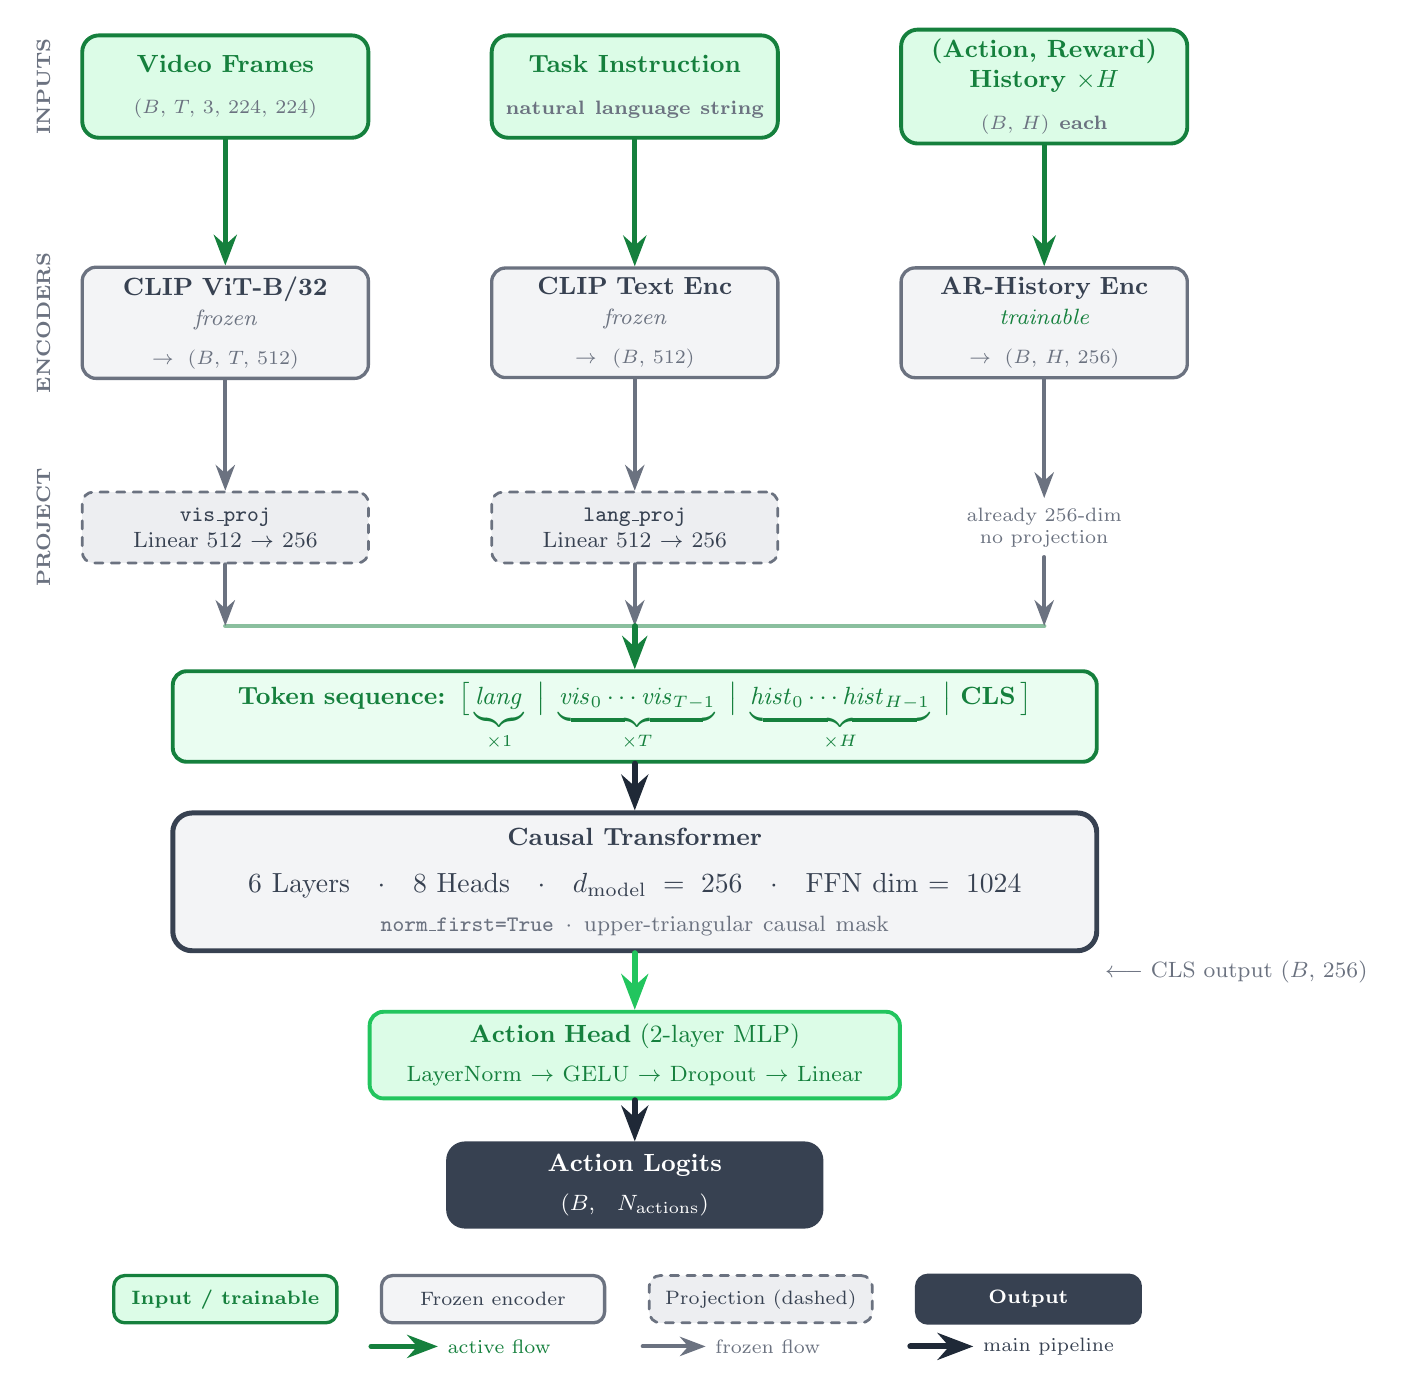
\begin{tikzpicture}[
  >=Stealth,
  every path/.style={line cap=round, line join=round},
]

%% ── Column x-positions ───────────────────────────────────────────────────────
\def\xL{-5.2}
\def\xC{0}
\def\xR{5.2}

%% ════════════════════════════════════════════════════════════════════════════
%%  ROW 1 — Raw inputs  (y = 0)
%% ════════════════════════════════════════════════════════════════════════════
\node[inp] (vid) at (\xL, 0)
  {Video Frames\\[4pt]{\scriptsize\color{DimGray}$(B,\,T,\,3,\,224,\,224)$}};
\node[inp] (lan) at (\xC, 0)
  {Task Instruction\\[4pt]{\scriptsize\color{DimGray}natural language string}};
\node[inp] (his) at (\xR, 0)
  {(Action, Reward)\\History $\times H$\\[4pt]{\scriptsize\color{DimGray}$(B,\,H)$ each}};

%% Section label
\node[font=\scriptsize\bfseries\color{DimGray}, left=0.3cm of vid.west]
  at (\xL-1.8, 0) {\rotatebox{90}{INPUTS}};

%% ════════════════════════════════════════════════════════════════════════════
%%  ROW 2 — Encoders  (y = -3.0)
%% ════════════════════════════════════════════════════════════════════════════
\node[enc] (venc) at (\xL, -3.0)
  {\textbf{CLIP ViT-B/32}\\{\footnotesize\itshape\color{DimGray}frozen}\\[3pt]%
   {\scriptsize\color{DimGray}$\to(B,\,T,\,512)$}};
\node[enc] (lenc) at (\xC, -3.0)
  {\textbf{CLIP Text Enc}\\{\footnotesize\itshape\color{DimGray}frozen}\\[3pt]%
   {\scriptsize\color{DimGray}$\to(B,\,512)$}};
\node[enc] (henc) at (\xR, -3.0)
  {\textbf{AR-History Enc}\\{\footnotesize\itshape\color{DarkGreen}trainable}\\[3pt]%
   {\scriptsize\color{DimGray}$\to(B,\,H,\,256)$}};

\node[font=\scriptsize\bfseries\color{DimGray}, left=0.3cm of venc.west]
  at (\xL-1.8, -3.0) {\rotatebox{90}{ENCODERS}};

%% ════════════════════════════════════════════════════════════════════════════
%%  ROW 3 — Projections  (y = -5.6)
%% ════════════════════════════════════════════════════════════════════════════
\node[prj] (vprj) at (\xL, -5.6)
  {\texttt{vis\_proj}\\Linear $512\!\to\!256$};
\node[prj] (lprj) at (\xC, -5.6)
  {\texttt{lang\_proj}\\Linear $512\!\to\!256$};
\node[font=\scriptsize\color{DimGray}, align=center] (hpass) at (\xR, -5.6)
  {already 256-dim\\no projection};

\node[font=\scriptsize\bfseries\color{DimGray}, left=0.3cm of vprj.west]
  at (\xL-1.8, -5.6) {\rotatebox{90}{PROJECT}};

%% ════════════════════════════════════════════════════════════════════════════
%%  Merge bar  (y = -6.85)
%% ════════════════════════════════════════════════════════════════════════════
\coordinate (mergeL) at (\xL,  -6.85);
\coordinate (mergeC) at (\xC,  -6.85);
\coordinate (mergeR) at (\xR,  -6.85);

\draw[color=DarkGreen!50, line width=1.6pt]
  (mergeL) -- (mergeR);

%% Arrows from projections down to merge bar
\draw[->, color=DimGray, line width=1.4pt] (vprj.south)  -- (mergeL);
\draw[->, color=DimGray, line width=1.4pt] (lprj.south)  -- (mergeC);
\draw[->, color=DimGray, line width=1.4pt] (hpass.south) -- (mergeR);

%% ════════════════════════════════════════════════════════════════════════════
%%  Token sequence box  (y = -8.0)
%% ════════════════════════════════════════════════════════════════════════════
\node[tokbox] (toknode) at (0, -8.0)
  {\textbf{Token sequence:}\enspace
   $\bigl[\,%
     \underbrace{\mathit{lang}}_{\times 1}\ \big|\ %
     \underbrace{\mathit{vis}_{0}\cdots\mathit{vis}_{T-1}}_{\times T}\ \big|\ %
     \underbrace{\mathit{hist}_{0}\cdots\mathit{hist}_{H-1}}_{\times H}\ \big|\ %
     \mathbf{CLS}%
   \,\bigr]$};

%% Arrow from merge bar center to token box
\draw[->, color=DarkGreen, line width=2pt] (mergeC) -- (toknode.north);

%% ════════════════════════════════════════════════════════════════════════════
%%  Causal Transformer  (y = -10.1)
%% ════════════════════════════════════════════════════════════════════════════
\node[fusbox] (trans) at (0, -10.1)
  {Causal Transformer\\[6pt]
   {\normalsize\mdseries
    6 Layers\quad$\cdot$\quad 8 Heads\quad$\cdot$\quad
    $d_{\mathrm{model}}=256$\quad$\cdot$\quad FFN dim $=1024$}\\[3pt]
   {\footnotesize\mdseries\color{DimGray}
    \texttt{norm\_first=True}\enspace$\cdot$\enspace
    upper-triangular causal mask}};

\draw[->, color=ArrowDark, line width=2.2pt] (toknode.south) -- (trans.north);

%% CLS readout side-label
\node[font=\footnotesize\color{DimGray}, right]
  at (5.85, -11.25) {$\longleftarrow$ CLS output $(B,\,256)$};

%% ════════════════════════════════════════════════════════════════════════════
%%  Action Head  (y = -12.3)
%% ════════════════════════════════════════════════════════════════════════════
\node[hdbox] (head) at (0, -12.3)
  {\textbf{Action Head} (2-layer MLP)\\[3pt]
   {\footnotesize LayerNorm $\to$ GELU $\to$ Dropout $\to$ Linear}};

\draw[->, color=MidGreen, line width=2.2pt] (trans.south) -- (head.north);

%% ════════════════════════════════════════════════════════════════════════════
%%  Output  (y = -13.95)
%% ════════════════════════════════════════════════════════════════════════════
\node[outbox] (aout) at (0, -13.95)
  {Action Logits\\[3pt]{\footnotesize$(B,\;N_{\mathrm{actions}})$}};

\draw[->, color=ArrowDark, line width=2.2pt] (head.south) -- (aout.north);

%% ════════════════════════════════════════════════════════════════════════════
%%  Input → Encoder arrows  (thick, dark green)
%% ════════════════════════════════════════════════════════════════════════════
\draw[->, color=DarkGreen, line width=1.8pt] (vid) -- (venc);
\draw[->, color=DarkGreen, line width=1.8pt] (lan) -- (lenc);
\draw[->, color=DarkGreen, line width=1.8pt] (his) -- (henc);

%% Encoder → Projection arrows  (gray)
\draw[->, color=DimGray, line width=1.4pt] (venc) -- (vprj);
\draw[->, color=DimGray, line width=1.4pt] (lenc) -- (lprj);
\draw[->, color=DimGray, line width=1.4pt] (henc) -- (hpass);

%% ════════════════════════════════════════════════════════════════════════════
%%  Legend  (bottom-left)
%% ════════════════════════════════════════════════════════════════════════════
\begin{scope}[shift={(-5.2, -15.4)}]
  \node[leg, draw=DarkGreen, line width=1.2pt, fill=FillGreen,
        font=\scriptsize\bfseries\color{DarkGreen}]        at (0,   0) {Input / trainable};
  \node[leg, draw=DimGray,   line width=1.2pt, fill=LightGray,
        font=\scriptsize\color{DarkGray}]                  at (3.4, 0) {Frozen encoder};
  \node[leg, draw=DimGray, dashed, line width=1pt, fill=MidGray!40,
        font=\scriptsize\color{DarkGray}]                  at (6.8, 0) {Projection (dashed)};
  \node[leg, draw=DarkGray, line width=1.4pt, fill=DarkGray,
        font=\scriptsize\bfseries\color{white}]            at (10.2, 0) {Output};
  %% Arrow samples
  \draw[->, color=DarkGreen, line width=1.8pt] (1.85, -0.6) -- (2.7, -0.6);
  \node[font=\scriptsize\color{DarkGreen}, right] at (2.7, -0.6) {active flow};
  \draw[->, color=DimGray, line width=1.4pt]   (5.3, -0.6) -- (6.1, -0.6);
  \node[font=\scriptsize\color{DimGray}, right] at (6.1, -0.6) {frozen flow};
  \draw[->, color=ArrowDark, line width=2.2pt] (8.7, -0.6) -- (9.5, -0.6);
  \node[font=\scriptsize\color{DarkGray}, right] at (9.5, -0.6) {main pipeline};
\end{scope}

\end{tikzpicture}
\end{document}
